% Indicate the main file. Must go at the beginning of the file.
% !TEX root = ../main.tex

%%%%%%%%%%%%%%%%%%%%%%%%%%%%%%%%%%%%%%%%%%%%%%%%%%%%%%%%%%%%%%%%%%%%%%%%%%%%%%%%
% 03_results
%%%%%%%%%%%%%%%%%%%%%%%%%%%%%%%%%%%%%%%%%%%%%%%%%%%%%%%%%%%%%%%%%%%%%%%%%%%%%%%%


\section{Results}
\label{results}

\subsection{Hyperparameter Tuning}%%%%%%%%%%%%%%%%%%%%%%%%%%%%%%%%%%%%%%%%%%%%%%

The detailed results of the Hyperparameter tuning are shown in \autoref{tab:hyperparameters_results}.
The ranking of the score according to the accuracy or the F1 score are similar but there are some differences.
The best performing model had and accuracy of 0.706 with an F1 score of 0.571, while 
the best model according to the F1 (0.608) score had an accuracy of 0.667.
It is quite difficult to find any obvious tendencies for the influence of the hyperparameters on the performance of the model.
\autoref{fig:hyperparameters_boxplot} shows the distribution of the accuracy comparing different different hyperparameters
grouped by the transformation used. There was a tendency visible for the MelSpectrogramm to work a bit better.
A smaller learning rate seems to deliver more robust results in general, yet the difference was marginal.
For the Mel spectrogram, the best performance was observed with 3 ResBlocks, while this hyperparameter had no impact with the standard spectrogram overall.
Furthermore, there was a tendency for smaller kernel sizes to deliver more robust results,
and the best performance was achieved with a kernel size of 5.

%==== figure: hyperparameters_boxplot ====%
\begin{figure}[h]
\centering
\captionsetup{width=0.9\linewidth}
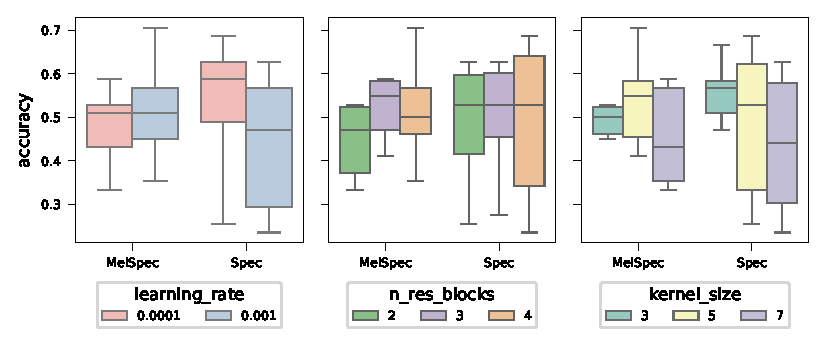
\includegraphics[width=1.0\textwidth]{figures/hyperparameters_boxplot.pdf}
\caption{Accuracy of the models for different hyperparameter grouped by the transformation type.}
\label{fig:hyperparameters_boxplot}
\end{figure}

%=========================================%

In \autoref{fig:hyperparameters_scatterplot}, the
models size measured by the number of trainable parameters is plotted against the accuracy and the F1 score.
There was no obvious correlation visible between the model size and the performance of the model.
This is also supported by the results of the Pearson Test. For both metrics, the p value was clearly above 0.05 
(the chosen confidence interval), i.e., the null hypothesis -- that there is no relationship between the performance and the number of model parameters -- had to be rejected.
The r values were both quite close to zero but negative, which indicates that there might be a slight -- yet not significant -- tendency for a smaller model to perform better.

%==== figure: hyperparameters_scatterplot ====%
\begin{figure}[h]
\centering
\captionsetup{width=0.9\linewidth}
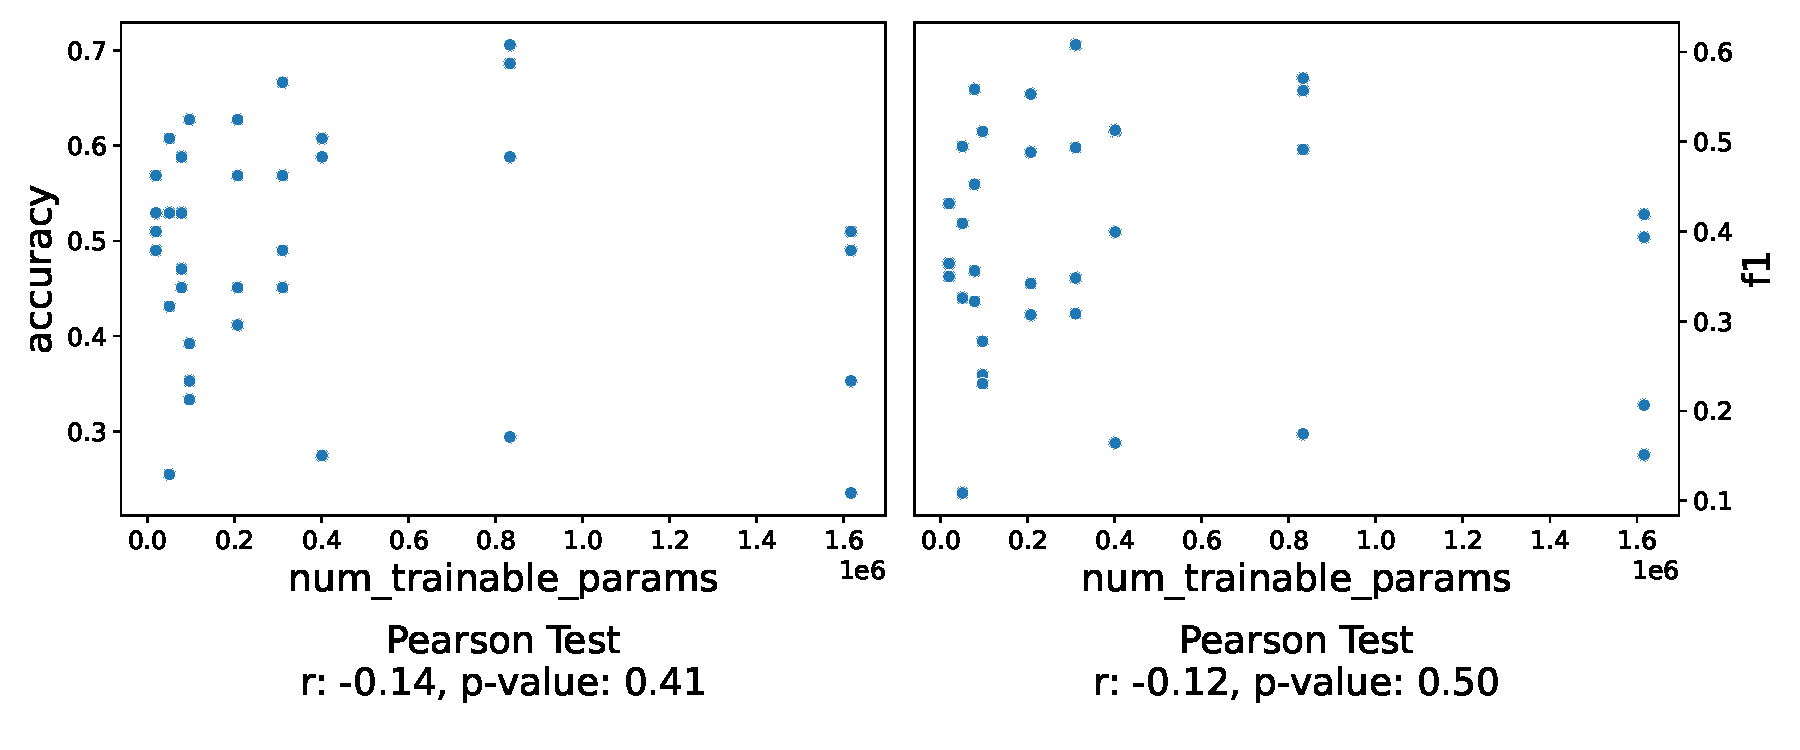
\includegraphics[width=1.0\textwidth]{figures/hyperparameters_scatterplot.pdf}
\caption{Model size compared to the accuracy and F1 Score of the models.}
\label{tab:hyperparameters_scatterplot}
\end{figure}

%=============================================%

The F1 score per class is shown in \autoref{fig:f1_per_class} and compared to the distribution
of the available data. Class 11 has a very low F1 score compared to the available data while class 9 has a very high F1 Score
compared to the available data. To further examine the relation between the F1 score and the distribution of the data
in \autoref{fig:f1_per_class_to_data_distribution}, the F1 score is plotted against the distribution of the training data.
There is no obvious correlation visible between the F1 score and the distribution of the data. This is also supported by the results
of the Pearson Test. The p value is above 0.05, i.e., we accept the null hypothesis that there is no significant relationship. The r value
is positive, and therefore, there might be a slight tendency for more training data to deliver a better F1 score.

%==== figure: f1_per_class ====%
\begin{figure}[h]
\centering
\captionsetup{width=0.9\linewidth}
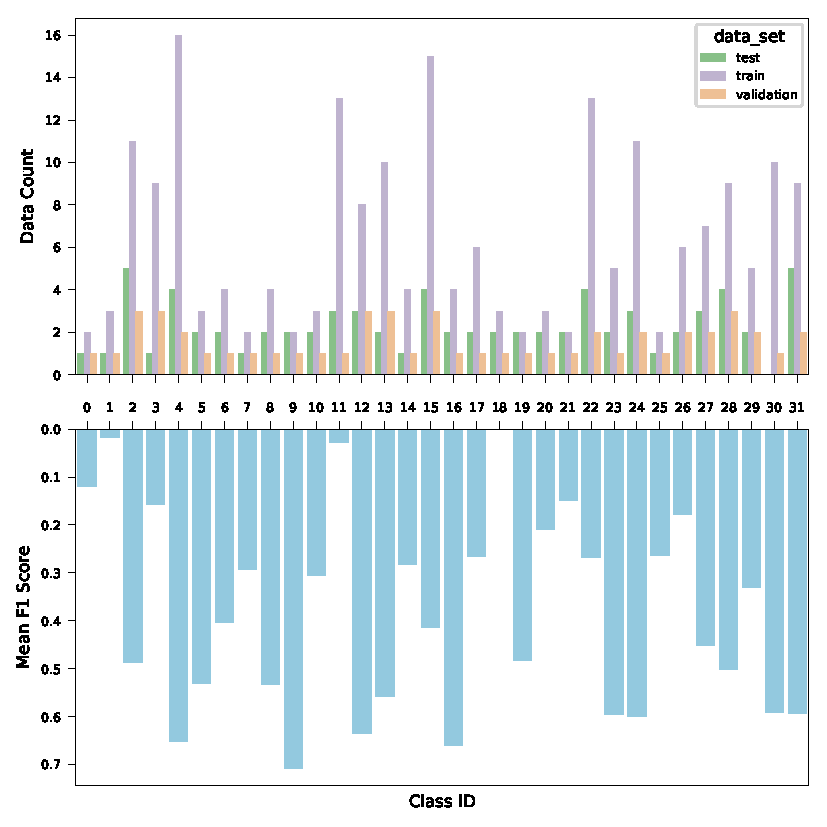
\includegraphics[width=1.0\textwidth]{figures/f1_per_class.pdf}
\caption{F1 Score per class as mean trough all models compared to data distribution.}
\label{tab:f1_per_class}
\end{figure}

%==============================%

%==== figure: f1_per_class_to_data_distribution ====%
\begin{figure}[h]
\centering
\captionsetup{width=0.8\linewidth}
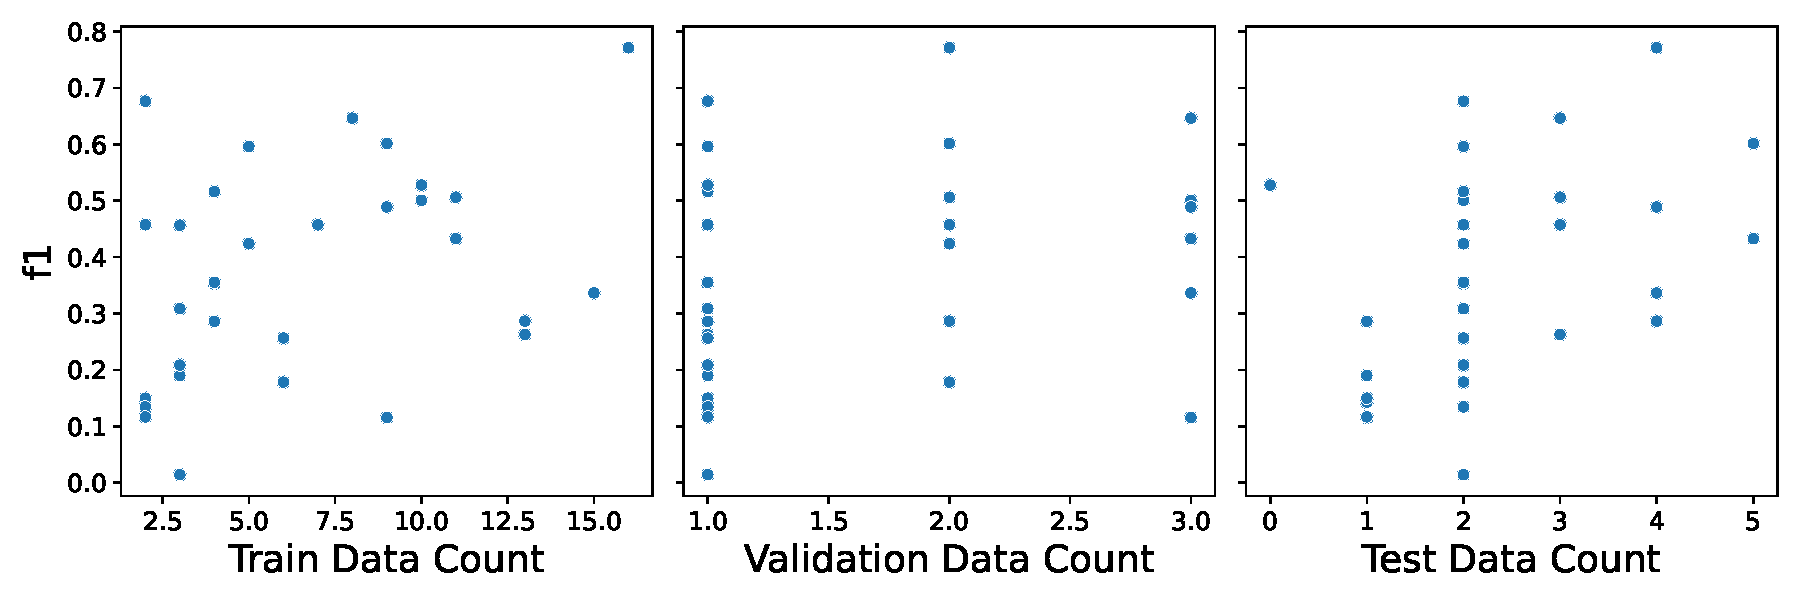
\includegraphics{figures/f1_per_class_to_data_distribution.pdf}
\caption{Available training data per classes compared to the F1 Score per classes in a scatter plot and the result of the Pearson correlation test.}
\label{fig:f1_per_class_to_data_distribution}
\end{figure}

%===================================================%


\subsection{Performance of the best Model}%%%%%%%%%%%%%%%%%%%%%%%%%%%%%%%%%%%%%%

The best performing configuration for the model was found to be the one with the following hyperparameters:

\begin{itemize}
    \item \textbf{n\_mels:} 64
    \item \textbf{n\_res\_blocks:} 4
    \item \textbf{learning\_rate:} 0.001
    \item \textbf{kernel\_size:} 5
\end{itemize}

On the test set, the model achieved an accuracy of 0.649 and an F1 score of 0.546. 
The confusion matrix for the predictions generated by this model is shown in \autoref{fig:confusion_matrix_best}.
The concentration of results in the diagonal of the confusion matrix indicates that the model is performing well.
Class 22 was predicted the most frequent with more than 50\% of the predictions being wrong.

%==== figure: confusion_matrix_best ====%
\begin{figure}[h]
\centering
\captionsetup{width=0.9\linewidth}
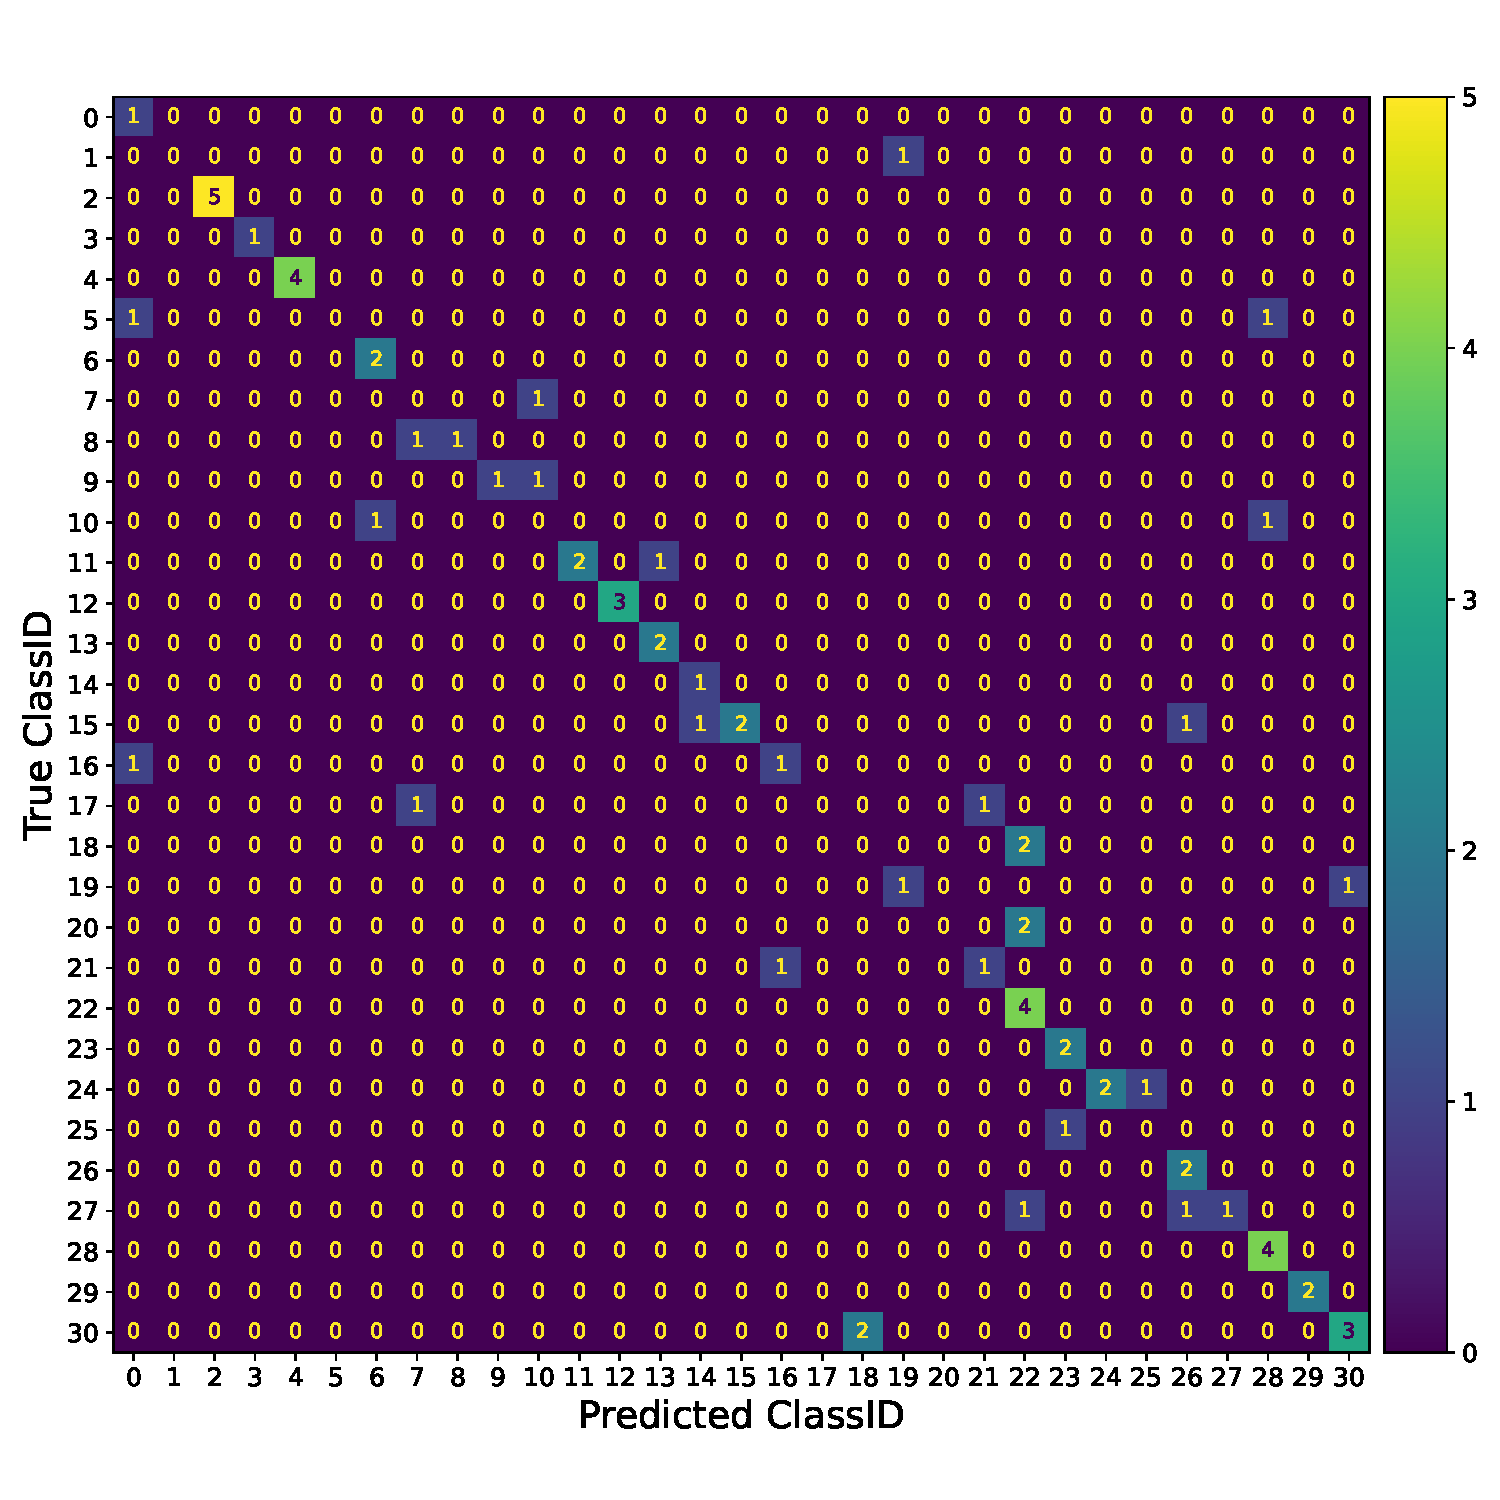
\includegraphics[width=1.0\textwidth]{figures/confusion_matrix_best.pdf}
\caption{Confusion matrix for the predictions of the test set using the best model. The over all accuracy on the test set was 0.649.}
\label{tab:confusion_matrix_best}
\end{figure}

%=======================================%

Next, we take a closer look at the training curves of the best-performing model. The validation accuracy and loss at the end of
every epoch is shown in \autoref{fig:loss_acc_best}. The graphs show a typical
training process. The validation accuracy is increasing while the validation loss
is decreasing. Towards the end, both graphs are flattening out which is a sign that
the model was not learning anymore when the training was stopped. This indicates that the patience
of 100 for the early stopping was an appropriate choice. Since the validation loss
and accuracy are very noisy, it was necessary to use a large patience value.

%==== figure: loss_acc_best ====%
\begin{figure}[h]
\centering
\captionsetup{width=0.9\linewidth}
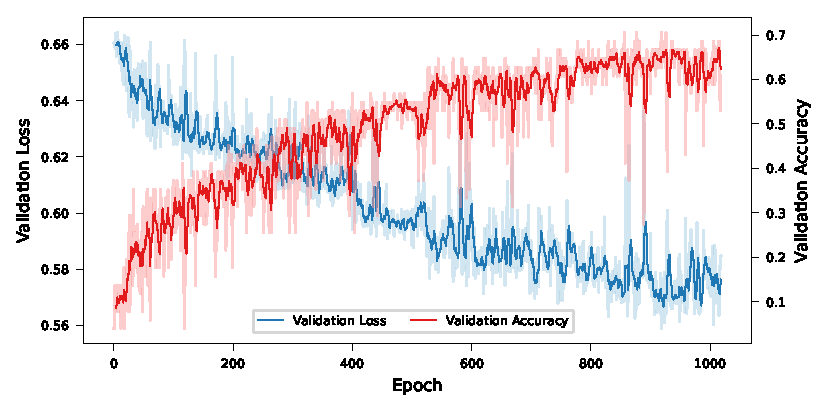
\includegraphics[width=1.0\textwidth]{figures/loss_acc_best.pdf}
\caption{The validation loss and accuracy of the best model. Light version is not smoothed and dark version is smoothed with a window size of 5.}
\label{tab:loss_acc_best}
\end{figure}

%===============================%
